\begin{subsection}{Background}

\begin{frame}{Background}
\begin{figure}
\begin{columns}%
        \begin{column}{0.8\textwidth}%
            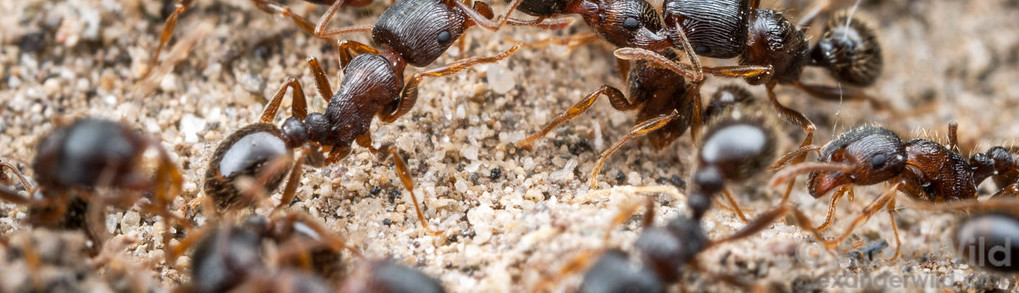
\includegraphics[width=\textwidth,right]{images/caespitum16j-XL}
        \end{column}%
        \begin{column}{0.2\textwidth}%
            \caption{\textit{Tetramorium caespitum} \scriptsize{\cite{alexander_wild_caespitum-16j-xl.jpg_????}}}
        \end{column}%
    \end{columns}
\end{figure}
The collective foraging behavior of ants is well studied, including
\begin{itemize}
	\item the strategies ants use to engage in foraging behavior {\scriptsize\cite{camazine_self-organization_2003}}
    \item how ants tend to select the shortest path to food {\scriptsize\cite{camazine_self-organization_2003}}
    \item how ants tend to select the richest food source {\scriptsize\cite{camazine_self-organization_2003}}
    \item approaches to mathematical modeling of ant foraging  {\scriptsize\cite{perna_individual_2012,ryan_model_2016}}
\end{itemize}

\end{frame}
\end{subsection}
